\def\baselinestretch{1}
\chapter{CONCLUSION AND FUTHER WORK}
\label{chap:Conclusiont}
\ifpdf
    \graphicspath{{Conclusions/ConclusionsFigs/PNG/}{Conclusions/ConclusionsFigs/PDF/}{Conclusions/ConclusionsFigs/}}
\else
    \graphicspath{{Conclusions/ConclusionsFigs/EPS/}{Conclusions/ConclusionsFigs/}}
\fi

\def\baselinestretch{1.66}

\section{Conclusion}

Based on the idea of biology research, we implemented an new motion synthesis framework.
We also introduce new mathematical tools for both the graphic motion synthesis research and biological motor control research.
by the idea of topology conjungacy, we unified the different biological idea.

our idea propose an computational efficient method for graphic research.

by the topolgy and symmery property,
the dynamic of system can be catagloryed.




\section{Futher Work}
Our research is not finished, based on the method we found, new question arise.
Which in our eyes are important for both the biological and graphic research.
\subsection{Local Frame Based Method}
In our method, the transformation is described by a fixed frame.
Through the idea of differential gemometry, transformation can also be described with moving frame or local frame.

Some invariant form is easy in local frame and symmetry direction can by decoupled in local frame.
this will provide us  some more types of symmetry which are hard to find in fixed method.

one example is the nohonomoilic dynamic system, which are not discussed in our research.


\subsection{Integrable System}

entrainmet and CPG only get the structual stability through emerical method.
For application use, we can use an analysoub but stable sytem instead of the original system.


A different idea is we start from a structural stable dynamic system and the modify it to approximate the cpg.
some idea for this maybe the integrable system and perturbation theoy.

by substitute the cpg with an disturbed integrable system may provide better 
\subsection{Symmetry of PDE}
we are very interesting in expand our method to the pde domain, if so, we can simulate motion involves fluid and elestic object.

\subsection{System Transform and Muscle Actuation}
One question we have not touched in our research is the muscle system.

in our research, our method is based on transform the state space.
this will result in a control method that need to accurately feedback the current state.

while a different idea is transform the dynamic system.
If the system is of High Dof, when we can achieve the same effect as controlled symmetry by modifying the system's parameters.

for the simple  mass spring system.
off set can implemented by chaning the rest length d
speed action can be implemented by chaning the stiffness K
 and energy scaling is met by the dyanmics, control can be achieved by ajust the stiffness K and then restore it.


this method will get rid of the need of feedback and extral control effort, which is more realistic to natual motor results.
In this point view, an controllable spring is avatange for energy shapping method.

this may give us some insight into our body's muscle system.
A further hypothsis muscle are not used to generating force, treat them as parameters that transfrom th system they can be seen as an advantage.

also when symmetry is applied, muscle system will change in an uniform manner.
this is the same with the biological idea of muscle synergy.

we try to incoporate muscles in the the following research, current problems is include more muscles will include more parameters and complicate the dynamic simulation.



\subsection{Perception Dynamics}
human motion perception is an high level capacity, basecall it is based up our object recoganition ability and our dynamic reasoning ability.
When dynamic motion synthesis, we also touch the question of dynamic perception and encoding problem in intelligence.

It is not very likely that the neural system encode the dynamic system in the form of symbolic differential equation.
while our approach in motor control provide two ideas for modeling dynamics in our neural system.

the first is qualitative approach.
Neural system may not need to encode the details of dynamic system, neural system can form an analous dynamic system in our brain that is analogys to the real dynamics.
Such model will like the details accuracy, but get the qualitatives properties right.

Another idea is we can remeber behaviour of one dynamic system, and appling transformation when we econter a different dynamic system.


we are not still not sure which method is better, but both of them are better than solving the differential equaiton in our brain.
We proprose maybe a new dynamic simulator can be designed by this principles, if neural system encode the dynamic in this way, we can expected that such kind of simulator will result in belieable motion and are more intutive for animators to use.It can be aslo be used as and tools to biological research.s
\subsection{Rethink abouth the uncanny valley}
For computer graphic research, uncanny valley is the central problem. Currently little is known about over comming the valley mainly because we don't yet know the mechanism behind.
although it is wiered in our research to apply to motor invaraint in our research,
our research may provide some insight in to the uncanny valley.

we propose that the uncanny phenomenon is because there is a switch of perception mechanism in human perception.
if we meet something not familar, our perception mechism is based analogy, which we only care about the qualitative properties,as long as the qualitative properties of it is similar to some qualitative propers of our known, we think it "belieable". This is extendion of our idea of Global Invariant.

if something is very like to something we know, we used a different perception mechanism, which is based on our experience.
Maybe we will begin to analysizing some quantative properties and measure the difference between the observed and our experience.
this can be seen as an extension of our idea of local invariant.


When the object is becomming more and more like in our experience, there is a switch in the perpection mechanism, the origianl qualitative analy ones become very poor alike in the quantative approach,
thus wil result in the valley.

This idea is just a propose and need further proof and experiment.
but we find it interesing and if so, maybe we will move into a new era of graphic research.


\begin{figure}[!htbp]
  \begin{center}
      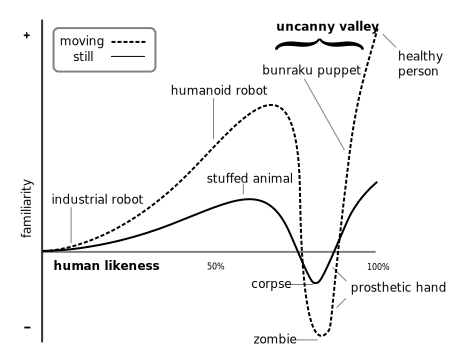
\includegraphics[width=0.5\textwidth]{Mori_Uncanny_Valley}
    \caption{Uncanny Valley}
    \label{fig:fishplot}
\end{center}
\end{figure}

%%% ----------------------------------------------------------------------

% ------------------------------------------------------------------------

%%% Local Variables: 
%%% mode: latex
%%% TeX-master: "../thesis"
%%% End: 
